% !TeX spellcheck = en_GB
\chapter{Sword handling}\label{ch:grip}

\paragraph*{}
In Chinese culture, swordsmanship and calligraphy are considered as intimately related arts.
It is commonly said indeed that a sword should be handled as if it were a calligraphy brush.
This statement will be clear to everyone has tried one's hand at Chinese calligraphy: in order to achieve a proper control of the strokes, the brush must be held firmly yet not too tightly so as to be connected to the centre of the calligrapher's body.
Any weakness or stiffness in the way the brush is handled will result in angular or wobbly strokes.

Similarly, when wielding a sword, a weak or stiff grip will hinder the fluidity of movements and the proper connection between the sword and the body, invariably resulting in clumsy and lifeless movements of the sword.
In swordplay, an improper grip precludes sensing, adapting and reacting efficiently to the opponent's movements. 

Since the way the hilt is gripped determines how tractable the sword is, an appropriate grip with the right alignment and a tensionless attitude are essential to achieve a good unity with the sword.

\section{The sword grip} \index{grip}
Of all the types of grips I experimented, I strongly recommend the one shown in figure \ref{fig:grip} for both routine practice and swordplay.

To take this grip, align your tiger's mouth, wrist and forearm with the blade then wrap your fingers around the middle part of the handle, between the two ferrules.
The thumb, middle and ring finger lock the grip at the very centre of the handle.
Both the index and little fingers remain free and participate to the precise control of the hilt position in the hand or allow loosening or tightening the grip.

\begin{figure}[ht]
	\centering
	\subfigure[]{\label{fig:grip}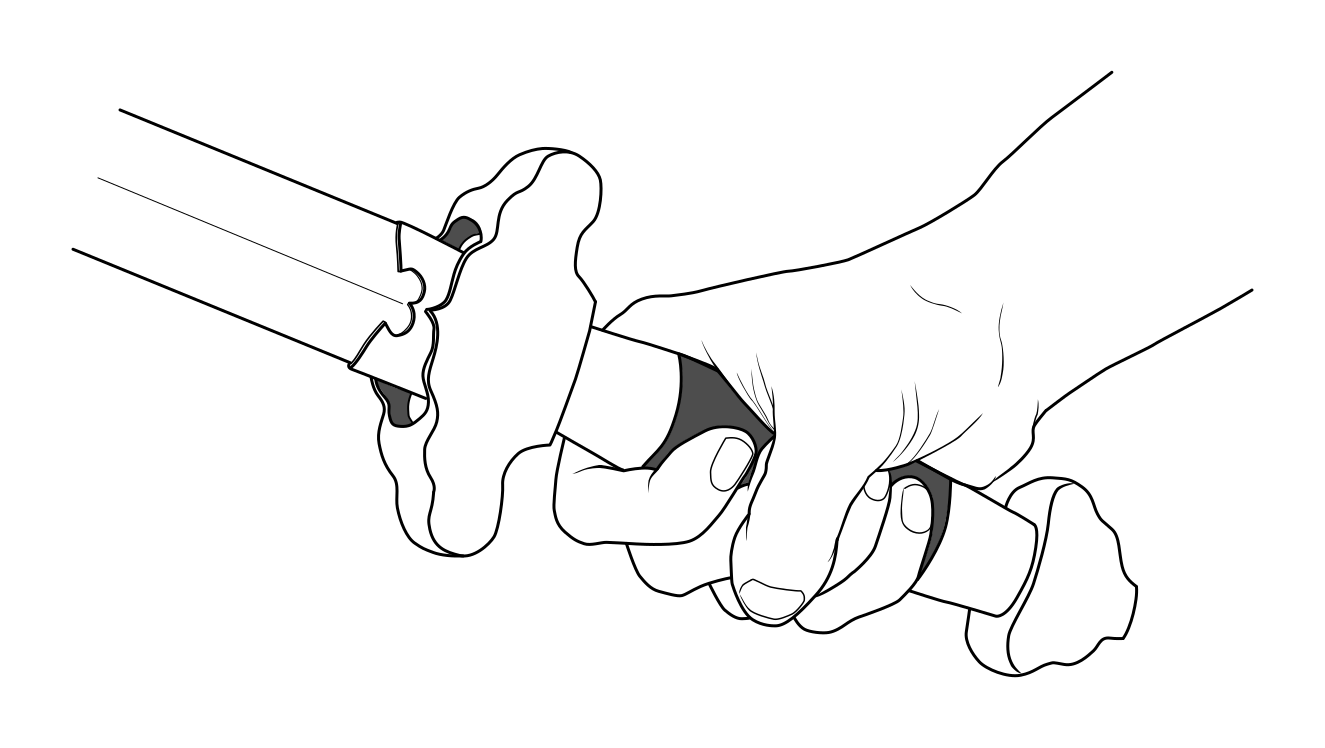
\includegraphics[width=0.69\textwidth]{../../Images/SwordGrip/sword_grip.pdf}}
	\subfigure[]{\label{fig:alignment}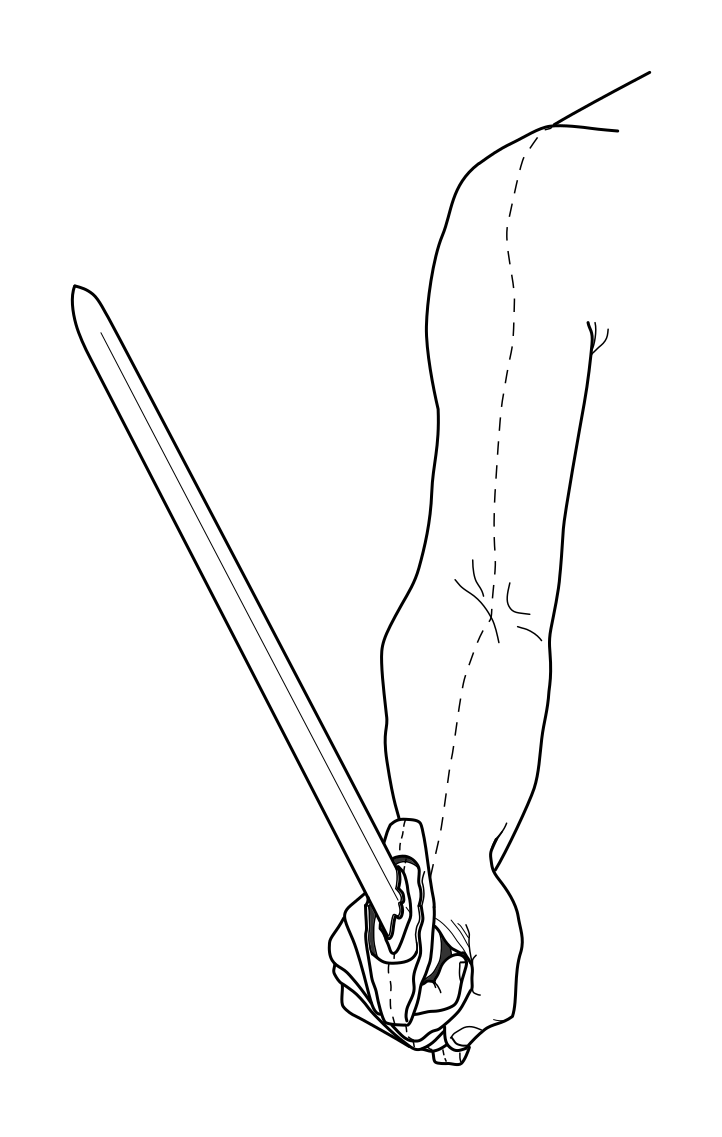
\includegraphics[width=0.29\textwidth]{../../Images/SwordGrip/alignment.pdf}}
	\caption[The sword grip]{The sword grip: \subref{fig:grip} the fingers are wrapped around the medium part of the handle with the thumb overlapping the middle and ring finger;
	\subref{fig:alignment} the wrist, elbow and shoulder joints are aligned with the blade as is represented by the dashed line.}
\end{figure}

As shown in figure \ref{fig:alignment}, the wrist, elbow and shoulder are aligned in the plane of the blade.\index{alignment}
This ensures that the sword is firmly rooted in the hand and that a good connection is achieved between the centres of the sword and the body, a prerequisite for efficient absorption and expression without tension nor strain on joints, muscles and sinews.
Furthermore, in this position, the elbow lies within the protective range of the guard and thus is less exposed to quick blows.

Occasionally, the grip may be adjusted to perform a particular technique, but when doing so, it is most important that much attention is paid not to heedlessly weaken nor stiffen the grip.
In any case, when the circumstances are not favourable for changing grip, which is often the case in free sparring, it is highly recommended to keep on with the main grip described above.

The sword  mobility is also controlled by tightening or loosening the grip. 
It should be reminded though that no finger should ever fully release the handle: even when whirling the sword, all fingers should always maintain some control on the handle. 

I am convinced that it is crucial to refrain from holding the handle next to the guard, even if the sword would feel less heavy this way because of the grip being closer to the sword's centre of gravity.

First of all, when the hand is at the centre of the hilt, the spindle-shaped handle fits the palm nicely and, as the guard and pommel are further away from the hand, they do not hinder sword movements.

Furthermore, Chinese guards being very narrow they do not wrap fully around the hand as the rapier's shell does and do not provide as much protection to the hand. However, if the grip is centred on the handle, the thumb and the forefinger are further away from the opponent's edge when controlling his blade and thus, are less exposed to accidental cuts than they would be with the hand next to the guard.

Finally, on a well-balanced\index{balance} sword, the centre of rotation resulting from a centred grip is precisely at the right location to enable the pommel to fully play its role in the sword dynamic balance\footnote{See chapter \ref*{ch:chinesesword} for more details on sword balance.}, ensuring swift and lively sword movements that can really make a difference in swordplay.

\section{The sword fingers}
The hand posture known as the \emph{sword fingers} or \emph{sword talisman} is definitely emblematic of Chinese straight sword practice and particularly of \Taijijian{}.
In its traditional version shown in figure \ref{fig:swordfingers}, the index and medium fingers are extended while the thumb, the ring and little fingers are connected to form a circle.
Some practitioners also use a more relaxed version where the thumb, the ring and little fingers are simply relaxed without assuming the form of a closed circle.

\begin{figure}[ht]
	\centering
	
\includegraphics[width=0.69\textwidth]{../../Images/SwordFingers/SwordFingers1.pdf}
	\caption[The sword fingers]{The sword fingers}
	\label{fig:swordfingers}
\end{figure}

The main role of the sword fingers is to create a spiral connecting the tip of the middle finger to the point of the blade and balancing the weight and movements of the sword.
This spiral is generated by stretching the left arm forward in a direction parallel to the line that passes through both tips of the extended fingers.

Although the spiral is effective with both the traditional and relaxed forms, the more constrained traditional one draws the attention more readily to the left side than does the relaxed version.

When beginners hold a sword, their mind is strongly focussed on the sword and their right hand. Very often, the other side of the body is left completely unattended unless they pay great attention to maintaining a proper sword fingers hand shape.
It is therefore important that beginners do not overlook the sword fingers.
It is only when they have gained sufficient experience and the balancing spiral has become natural that they may start using the relaxed form.

\section{Wielding the sword}
It is often repeated that the sword should be an extension of the body and that the practitioners should make one with their sword.
Although this may seem quite clear, it is far from being evident in practice.
First of all, the sword should be considered as an extra segment of the arm with the grip playing the role of an additional joint.
Like any other joint, the grip should therefore be relaxed and moving in unison with the whole body, allowing the sword to move freely in the hand.

If unity with the sword is purposed indeed, the sword nonetheless has its own individuality and its own particular way of responding to the practitioner's movements that depends on its physical characteristics.
It is therefore indispensable that the sword's individual demeanour should be acknowledged in order to blend harmoniously its movements with those of the practitioner.

This is somehow similar to dancing: a good dancer does not merely impose steps on his partner but is constantly aware of her position and thus is able to adapt to her moves and gently lead her to take the appropriate steps for the next figure. 
The same stands when wielding a sword.
Movements should not be imposed on the sword but the sword should be guided towards the appropriate direction to achieve the desired technique.
In return, the practitioner's movements and steps are guided by the sword's weight and impetus: if the sword is an extension of the body indeed, the body is nonetheless an extension of the sword...

There is a constant two-way exchange between the sword and the practitioner that is most apparent in routine practice but is no less important in free play.
Thus, even a rather heavy sword may be wielded effectively and swiftly with only a minimum of physical strength involved, the momentum of each movement being recovered and recycled into the next one.

The energy required to perform the techniques is provided by the weight and momentum of the sword itself combined with the right impulse from the body at the appropriate time.
Thanks to inertia, the sword's centre of gravity, borne along by the sword's momentum, acts as a fulcrum to allow increasing the speed of the tip or pointing it to another direction.
In free play, pressures exerted voluntarily or not by the opponent on the blade may also be absorbed, assimilated and transformed to generate attacks and ripostes.

To make a long story short we will conclude by saying that the energy is rooted in the hilt, controlled by the sword's centre and expressed in the blade.
